Hector Quadrotor เป็น ROS stacks (stack เป็นการรวบรวม packages ที่มีหลากหลายฟังก์ชันเอาไว้ด้วยกัน)
โดยภายในประกอบไปด้วย ROS packages ดังต่อไปนี้
\begin{enumerate}[label=\arabic*), leftmargin=1.5cm]
	\setlength\itemsep{-0.25em}
	\item hector\_quadrotor\_description
	\item hector\_quadrotor\_gazebo
	\item hector\_quadrotor\_teleop
	\item hector\_quadrotor\_gazebo\_plugin
\end{enumerate}


% \paragraph*{}
% เป็นแพกเกจที่มีไฟล์ quadrotor URDF model หลากหลายประเภท
% \paragraph*{hector\_quadrotor\_gazebo}
% เป็นแพกเกจที่มีไฟล์ launch สำหรับการทำ simulation ด้วยโปรแกรม Gazebo
% \paragraph*{hector\_quadrotor\_teleop}
% เป็นแพกเกจที่มีไฟล์ node สำหรับควบคุม quadrotor ด้วย gamepad
% \paragraph*{title}

\subsection{hector\_quadrotor\_description}
package นี้ให้ URDF model ของ quadrotor มี visual geometry เป็นไฟล์ COLLADA และ collision geometry เป็นไฟล์ STL
โดยจะเป็นส่วนเสริมที่ทำให้เราสามารถที่จะใช้ model ในโปรแกรม Gazebo ได้\footnote{http://wiki.ros.org/hector\_quadrotor\_description}

% \vspace{20pt}
\paragraph*{quadroter\_base.urdf.xacro}
เป็นไฟล์ xacro ของโมเดลขั้นพื้นฐานของ quadroter
\paragraph*{quadrotor.urdf.xacro}
เป็นไฟล์ xacro สำหรับการแสดงโมเดลขั้นพื้นฐานโดยไม่มีเซนเซอร์เพิ่มเติม
\paragraph{quadrotor\_hokuyo\_utm30lx.urdf.xacro}
เป็นไฟล์ xacro สำหรับการแสดงโมเดลขั้นพื้นฐานโดยเพิ่มเติมเซนเซอร์ Hokuyo เข้าไปสำหรับแสกนสิ่งแวดล้อม

\begin{figure}[!ht]
	\centering
	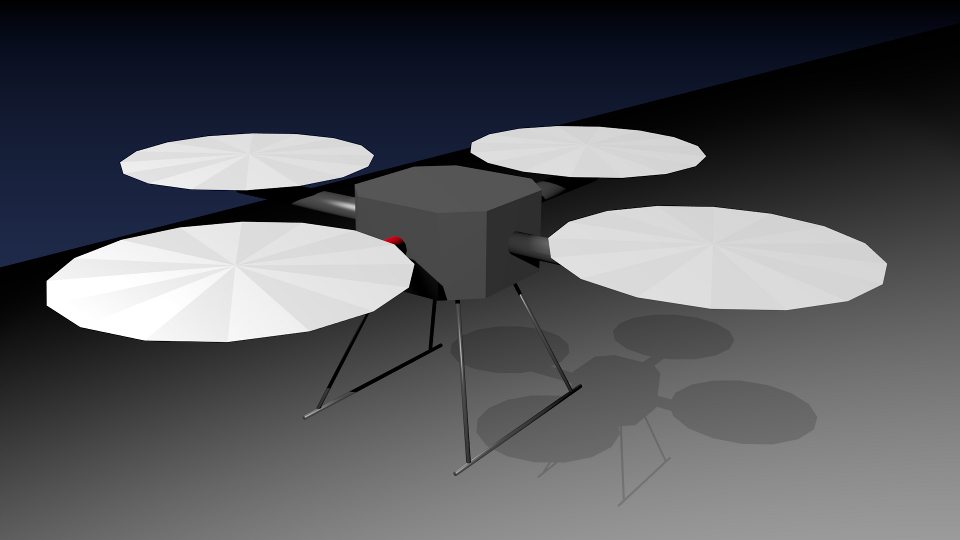
\includegraphics[width=0.85\textwidth]{images/hector_quadrotor_render.png}
	\caption{ภาพ quadrotor ที่ render ด้วย Blender}
	\label{fig:hector_quadrotor_render}
\end{figure}

\subsection{hector\_quadrotor\_gazebo}
package นี้ให้ quadroter model ที่มาจากไฟล์ urdf และมาแสดงผลในโปรแกรม Gazebo โดย features\footnote{http://wiki.ros.org/hector\_quadrotor\_gazebo} ที่มีคือ
\begin{enumerate}[label=\arabic*), leftmargin=1.5cm]
	\setlength\itemsep{-0.25em}
	\item Colored COLLADA quadrotor mesh model (.dae)
	\item URDF description
	\item Publishing of ground truth pose and simulated imu data
	\item Spawnable in Gazebo
	\item Controller สำหรับใช้ใน Gazebo โดยสามารถควบคุมผ่าน geometry\_msgs/Twist message ใน topic 'cmd\_vel'
\end{enumerate}

\clearpage
\subsection{hector\_quadrotor\_teleop}
package นี้จะทำให้เราสามารถที่จะควบคุม quadrotor ผ่าน gamepad ได้ โดยจะมี node ที่ publish geometry\_msgs/Twist message ไปที่ topic 'cmd\_vel'
ปัจจุบันมี gamepad 2 ชนิดที่นำมาใช้ได้ก็คือ
\begin{enumerate}[label=\arabic*), leftmargin=1.5cm]
	\setlength\itemsep{-0.25em}
	\item logitech\_gamepad.launch สำหรับ Logitech gamepads
	\item xbox\_controller.launch สำหรับ Xbox controller gamepads 
\end{enumerate}
แต่หากต้องการใช้งานนอกเหนือจากนี้ สามารถที่จะสร้าง node ขึ้นมาใหม่ได้

\vspace{20pt}
\subsection{hector\_quadrotor\_gazebo\_plugin}
package นี้เป็นส่วนเสริมของ Gazebo ที่จะทำให้มีเซนเซอร์ต่างๆเข้ามาในระบบได้
\paragraph*{Barometer Plugin}
เป็นส่วนเสริมที่จำลองเซนเซอร์ัที่ใช้วัดความสูงของ quadrotor โดยมีพื้นฐานมาจากการวัด barometric pressure
\paragraph*{Simple Controller Plugin}
package นี้เป็นส่วนเสริมของ Gazebo ที่จะทำให้เราสามารถควบคุม Velocities และ Yaw rate ได้โดยการคำนวณ แรงและแรงบิด
โดยในปัจจุบันยังไม่สามารถที่จะควบคุมตำแหน่ง ทิศทางการหันหัว และความสูงได้ แต่สามารถที่จะเขียนทับเข้าไปได้
\paragraph*{Quadrotor Propulsion Plugin / Quadrotor Aerodynamics Plugin}
package นี้เป็นส่วนเสริมของ Gazebo ที่จะทำให้เราสามารถควบคุมการหมุนของใบพัด quadroter ได้ โดยการควบคุม voltages ของมอเตอร์
และยังจำลอง wind vector ได้อีกด้วย
\paragraph*{Matlab Compilation}
ในการเขียนสมการต่างๆของระบบ quadroter มักจะนิยมใช้ Matlab script และคอมไพล์เป็น C libraries โดยใช้ Matlab Coder
ส่วนเสริมตัวนี้จะช่วยทำให้สามารถเชื่อมต่อกับ Matlab ได้

\begin{figure}[!ht]
	\centering
	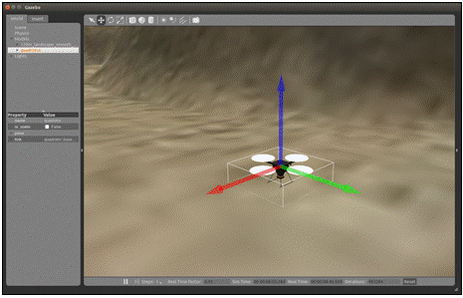
\includegraphics[width=0.85\textwidth]{images/hector_quadrotor_gazebo.png}
	\caption{ภาพ quadrotor ในโปรแกรม Gazebo}
	\label{fig:hector_quadrotor_gazebo}
\end{figure}